\section{Introduction}

\XXXnote{GWA : TODO : Rewrite proposal text.}

Redesigning the hardware-software interface will allow next generation
smartphones to effectively allocate energy between components and across time
to meet application needs. Improving performance, however, also requires
prioritizing energy usage to ensure that important applications receive the
resources they need to operate effectively, while recognizing that users use
their phones and applications different and will require different policies.
A user that only charges their phone at night, for example, requires
different energy management strategies than one that charges their phone
regularly at their desk or in the car.

Two major challenges stand in the way of an effective energy management
framework for smartphones. First, while measuring application energy usage
has received a great deal of attention, putting usage into context has not.
Measurement alone may provide helpful feedback to users, but is not
sufficient to enable effective policies, since the behavior and efficiency of
different applications varies, as does their importance to each user. It is
no surprise, for example, that an application like Skype consumes more energy
than a simple messaging client. And this information is not useful on its
own, since Skype's high energy usage might be acceptable if it is often used
and valued and unacceptable if it is not. These uncertainties make energy
usage alone usable for human interpretation---since users can use their own
experience to put the numbers in context---but \textit{unusable} for
automated response or application energy prioritization.

The second challenge is the fact that tuning energy consumption currently
requires deep integration with the specifics of each particular hardware
component, making writing cross-device policies difficult or impossible. A
policy that relies on a certain feature of a Wifi chipset available on a
particular device will fail on a second device if its Wifi driver fails to
support the feature. Without a narrow waste enabling cross-device policies,
energy management improvements will be limited to similar devices and quickly
become obsolete given the rapid improvements in smartphone technologies.

We propose to address both of these challenges through an cross-device energy
management policy framework called \textit{Jouler}. Jouler's policy engine
takes per-application energy measurement and utility determinations and uses
them to select application-specific inefficiency targets. The tuning
component then adjusts component-specific settings to meet the selected
inefficiency target, utilizing the interface improvements achieved by the
redesign objective previously described. To allow policies to be easily moved
between devices, policies do not operate on specific hardware components
directly. Instead, the operate on what we refer to as \textit{idealized
components}, which provide smooth tradeoffs between energy and one of several
performance metrics such as throughput, latency, or fidelity. To be
integrated into Jouler, specific components must translate operations on
these idealized components to adjustments appropriate for their particular
hardware device. Below we describe the two novel contributions of the Jouler
framework---determining application utility and utilizing idealized
components---before describing several possible Jouler policies.

\begin{figure*}
  
  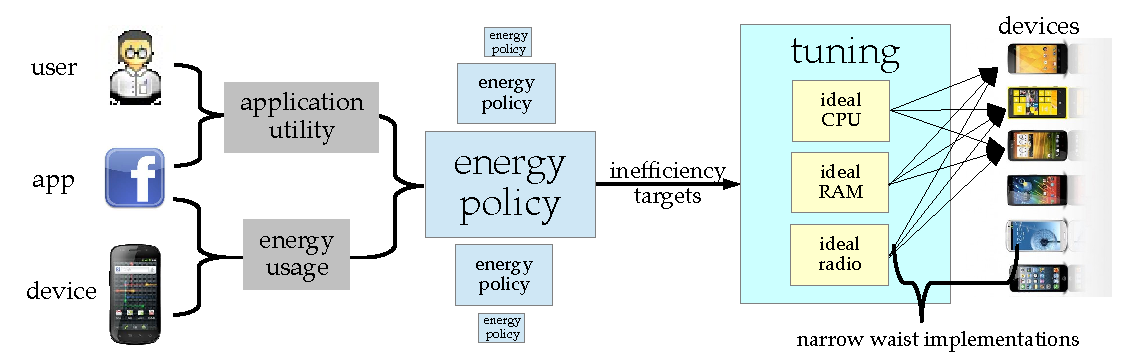
\includegraphics[width=\textwidth]{./figures/jouler.pdf}

  \caption{\textbf{The Jouler energy management policy framework.} Jouler
  addresses two key weaknesses of current smartphone energy management: lack
  of context for application energy usage and inability to write effective
  cross-device policies.}
  
  \vspace*{0.1in}
  \hrule
  \vspace*{-0.1in}
  \label{figure-jouler}

\end{figure*}
